% Publication-Grade Causal DAG: Collider Conditioning (Bad Control)
% Adheres to Pearl (2009) and Angrist and Pischke (2009)
% Compile with pdflatex or lualatex

\documentclass[tikz,border=10pt]{standalone}
\usepackage{tikz}
\usetikzlibrary{arrows.meta,positioning,shapes.geometric}

\begin{document}
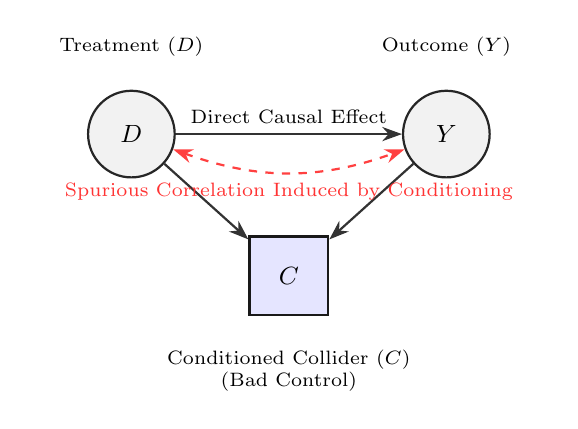
\begin{tikzpicture}[
    node distance=2.2cm and 2.5cm,
    every node/.style={font=\sffamily\small},
    observed/.style={circle, draw=black!85, fill=black!5, thick, minimum size=1.1cm},
    conditioned/.style={rectangle, draw=black!90, fill=blue!10, thick, minimum size=1.0cm},
    edge/.style={->, >={Stealth[length=2.5mm, width=1.8mm]}, thick, draw=black!80},
    spurious/.style={<->, >={Stealth[length=2.5mm, width=1.8mm]}, thick, dashed, draw=red!75}
]

    % Nodes
    \node[observed] (D) at (0, 0) {$D$};
    \node[observed] (Y) at (4.0, 0) {$Y$};
    \node[conditioned] (C) at (2.0, -1.8) {$C$};

    % Directed edges into collider
    \draw[edge] (D) -- (C);
    \draw[edge] (Y) -- (C);
    \draw[edge] (D) -- node[above, font=\scriptsize] {Direct Causal Effect} (Y);

    % Induced spurious association upon conditioning on C
    \draw[spurious] (D) to[bend right=20] node[below, font=\scriptsize, text=red!80] {Spurious Correlation Induced by Conditioning} (Y);

    % Node labels
    \node[above=0.3cm of D, text width=2.4cm, align=center, font=\scriptsize] {Treatment ($D$)};
    \node[above=0.3cm of Y, text width=2.4cm, align=center, font=\scriptsize] {Outcome ($Y$)};
    \node[below=0.3cm of C, text width=3.4cm, align=center, font=\scriptsize] {Conditioned Collider ($C$)\\ (Bad Control)};

\end{tikzpicture}
\end{document}
